\documentclass[draftcls, onecolumn, journal]{IEEEtran}
% \documentclass[journal]{IEEEtran}
% \documentclass[inproceedings]{article}
%\usepackage{fullpage}

%\renewcommand{\baselinestretch}{1.9}
\usepackage{graphicx}
%\usepackage{cite}
\usepackage[style=ieee, nohashothers=true, nosortothers=true, uniquelist=true, natbib=true, backend=biber, sorting=none]{biblatex}
\DefineBibliographyStrings{english}{andothers={}}

\addbibresource{project.bib}
\DeclareFieldFormat[article]{volume}{Vol. #1}
\DeclareFieldFormat[article]{number}{No. #1}
\DeclareFieldFormat[article]{pages}{p. #1}
\DeclareFieldFormat[inproceedings]{pages}{p. #1}

%\documentclass[journal]{IEEEtran}
\usepackage[a4paper, total={6in, 8.5in}, top=1in, bottom=1in, left=1in, right=1in]{geometry}
\usepackage{mathtools}
\usepackage{amssymb}
\usepackage{amsmath}
\usepackage{pythonhighlight}
\usepackage[utf8]{inputenc}
\usepackage{fancyhdr}
\usepackage{pythonhighlight}
\usepackage{changepage}
\usepackage{slashbox}
\usepackage{floatrow}
\usepackage{listings}
\usepackage[hidelinks]{hyperref}
\usepackage[T1]{fontenc}
\usepackage[utf8]{inputenc}
\usepackage[english]{babel}
\usepackage{csquotes}
\usepackage{booktabs}
\usepackage{multicol}
\usepackage{titlesec}
\usepackage{fontawesome5}
\usepackage{makecell}
\usepackage{footnote}
\usepackage{hyperref}

\setcounter{secnumdepth}{4}
\setcounter{tocdepth}{4}


\titleformat{\paragraph}
{\normalfont\normalsize\bfseries}{\theparagraph}{1em}{}
\titlespacing*{\paragraph}
{0pt}{3.25ex plus 1ex minus .2ex}{1.5ex plus .2ex}

\usepackage{caption}
\usepackage{subcaption}
\usepackage{color} %red, green, blue, yellow, cyan, magenta, black, white
\definecolor{mygreen}{RGB}{28,172,0} % color values Red, Green, Blue
\definecolor{mylilas}{RGB}{170,55,241}


\floatsetup[table]{capposition=top}

\sloppy
\definecolor{lightgray}{gray}{0.5}
\setlength{\parindent}{0pt}
\setlength{\headheight}{14pt}

\renewcommand{\headrulewidth}{.4mm} % header line width
\newcommand{\norm}[1]{\left\lVert#1\right\rVert}
\renewcommand\footnoterule{\kern-3pt \hrule width 3in \noindent \kern 2.6pt}


\pagestyle{fancy}
\fancyhf{}
\fancyhfoffset[L]{1cm} % left extra length
\fancyhfoffset[R]{1cm} % right extra length
\rhead{\bfseries Kutay U\u{g}urlu 2232841}
\lhead{ADPC for Tikhonov Regularization Parameter Choice}
\rfoot{}

\DeclarePairedDelimiter\ceil{\lceil}{\rceil}
\DeclarePairedDelimiter\floor{\lfloor}{\rfloor}

\author{Kutay U\u{g}urlu 2232841}

\begin{document}

    
\lstset{language=Matlab,%
    %basicstyle=\color{red},
    breaklines=true,%
    morekeywords={matlab2tikz},
    keywordstyle=\color{blue},%
    morekeywords=[2]{1}, keywordstyle=[2]{\color{black}},
    identifierstyle=\color{black},%
    stringstyle=\color{mylilas},
    commentstyle=\color{mygreen},%
    showstringspaces=false,%without this there will be a symbol in the places where there is a space
    numbers=left,%
    numberstyle={\tiny \color{black}},% size of the numbers
    numbersep=9pt, % this defines how far the numbers are from the text
    emph=[1]{for,end,break},emphstyle=[1]\color{red}, %some words to emphasise
    %emph=[2]{word1,word2}, emphstyle=[2]{style},    
}

\fancyfoot[C]{\thepage}

\title{\LARGE \LARGE EE798 Remote Image Formation Theory Project \newline \newline
Analysis and Reimplementation of \newline \textit{Improving the spatial solution of electrocardiographic
imaging: A new regularization parameter choice
technique for the Tikhonov method}}

\maketitle{\LARGE}
\pagebreak
\tableofcontents
\listoffigures
\listoftables
\pagebreak

\section{Introduction}\label{sec:intro}

\indent Electrocardiographic Imaging (ECGI) is a noninvasive method for reconstructing the epicardial potentials from the body surface potential mapping that can diagnose diseases such as tachycardia \cite{intini2005electrocardiographic} and atrial fibrillation \cite{figuera2016regularization,schuler2017ecg}. The number of measurement non-invasively taken from the torso surface, however, is less than the number of reconstructed cardiac sources that provides satisfactory spatial resolution for the diagnosis. Due to the inherent ill-posedness of this underdetermined problem, utilization of regularization is mandatory to achieve physiologically suitable solutions \cite{milanivc2014assessment}. Tikhonov Regularization is a widely used regularization technique in ECGI community and has been found to outperform the other methods depending on the formulation of the problem \cite*{milanivc2014assessment}. The regularization technique imposes a prior on the inverse problem solution and weights the candidate solutions with the data-fidelity term in the cost function with a regularization parameter $\lambda$. Chamorro-Servent, \textit{et al.}, proposes a new method called Automated Discrete Picard Condition(ADPC) in their study \cite*{chamorro2017improving} to automatically find a suitable regularization parameter $\lambda$. 
This project report investigates the idea reported in \textit{Improving the spatial solution of electrocardiographic
imaging: A new regularization parameter choice technique for the Tikhonov method}~\cite{chamorro2017improving}.  
\\
\\
The organization of the report is as follows:
\begin{itemize}
    \item The problem and the proposed solutions to it are briefly introduced in this section.
    \item The background of ECGI and theory of the regarding inverse problem are discussed in Section \nameref{sec:theory}.
    \item The methods, datasets and the details regarding the implementation of proposed methods for both the original study and the reimplemented version with another experimental setup are shared in the \nameref{sec:implementation} section.
    \item Section \nameref{sec:discussion} is left for the presentation of the results from conducted experiments along with the original results presented in the study and the discussion comparing the performances of the related method.
\end{itemize}

\newpage

\section{Theory}\label{sec:theory}

\begin{figure}[h]
    \centering
    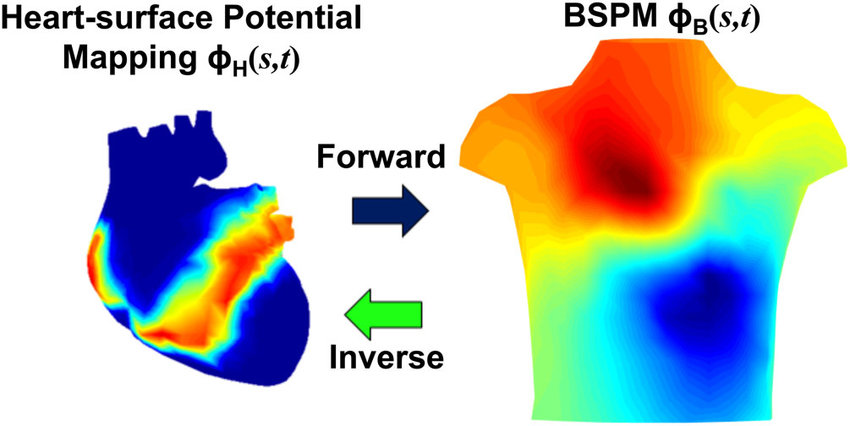
\includegraphics[width=0.8\textwidth]{../images/The-illustration-of-forward-and-inverse-ECG-problems.png}
    \caption{ECGI Forward and Inverse Problem}\label{fig:ECG}
\end{figure}

\subsection{ECGI Forward Problem}\label{subsec:ecgfor}

\indent ECGI Forward problem is constructing a model for calculating the body surface potential mapping(BSPM) from the given heart potentials, \textit{i.e.}, the epicardial voltage distribution, shown by the right-side arrow in Figure \ref{fig:ECG}. One can come up with different forward models for the ECGI problem. The authors of the original study utilized Method of Fundamental Solutions(MFS) method to derive the forward model, whereas Boundary Element Method(BEM) is utilized for the re-implementation. 

\subsubsection{Method of Fundemental Solutions} \label{subsec:MFS}
\indent MFS is meshless approach adapted to ECGI problem by Chamorro \textit{et al}. In this method, the measurements are expressed as a linear combination of fundamental solutions to the Laplace equation \cite*{wang2006application}. It is formulated as

\begin{equation}
    \Phi (x) = a_0 + \sum\limits_{j=1}^{N_s} f(x-y_j)a_j
    \label{eq:MFS}
\end{equation}

where $x \in \Omega$ where $\Omega$ is the measurement domain (torso) and $y_j$'s are the $N_s$ locations of the sources ($y_j \notin \Omega$) (heart). In this formulation $f$ stands for the fundamental solution to Laplace equation in Eqn. \eqref{eq:FundSoln}:

\begin{equation}
    f(r) = \frac{1}{4\pi} \frac{1}{|r|}
    \label{eq:FundSoln}
\end{equation}

After the discretization of the domain on torso measurement locations, the following system matrix M can be obtained:

\begin{center}
    $M = \begin{bmatrix} 
        1 & f(r_{11}) & \dots & f(r_1 N_S) \\
        \vdots & \vdots  & \ddots & \vdots\\
        1 &  f(r_{N_T1}) & \dots & f(r_{N_T} N_S) \\ 
        0 & \partial_{n_1}f(r_{11}) & \dots & \partial_{n_1}f(r_1 N_S) \\
        \vdots & \vdots  & \ddots & \vdots\\
        0 &  \partial_{n_{N_T}}f(r_{N_T1}) & \dots & \partial_{n_{N_T}}f(r_{N_T} N_S)     
        \end{bmatrix}$    
\end{center}

The coefficients belonging the above $N_T$ equations in the system equations satisfy the Dirichlet conditions, \textit{i.e.}, $\Phi$ = $\Phi_{T}$ on the torso measurement locations. Remaining coefficients represent the homogenous Neumann condition $(\partial \phi_n = 0)$. Therefore, the resulting system ends up with $Ma = b$, where $a$ is the $N_S + 1$ source coefficients and b = $\big(\begin{smallmatrix}
    \Phi_T \\
    0 
  \end{smallmatrix}\big)$  is the measurement vector representing the recorded potentials and no-flux condition. 

\subsubsection{Boundary Element Method}

Another possible forward model generation choice is the Boundary Element Method. BEM utilizes the discretization of the triangular boundary elements to solve the integral equations in a volume conductor also taking the conductivity distribution of the medium between the source and measurement domains into account \cite*{4536071}. To accurately generate the BSPM from epicardial surface potentials, an inhomogeneous heart-lungs-torso model is utilized in the model generation via BEM. In the reimplementation of the study BEM is used to generate both forward and inverse models. 

\subsection{ECGI Inverse Problem}\label{subsec:ecginv}

The aim of the ECGI inverse problem is to reconstruct the unknown epicardial surface potentials from the measured torso potentials. To diagnose the cardiac diseases such as infarction, the reconstructed potential mapping on the heart should have a satisfactory level of spatial resolution, \textit{i.e.}, the number of reconstruction points should be chosen dense enough. Since number of the torso potentials is usually much less than the number of cardiac source intensities, the problem is an underdetermined problem. That is, multiple different epicardial source configurations can result in the same torso measurement, even without the noise. In addition to this, the problem is highly ill-posed due to the physical nature of the volume conductor between the domains, which applies a low-pass effect on the BSPM. These are the most common factors that drastically affect the accuracy of the reconstructed solution in the ECGI inverse problem:

\begin{itemize}
    \item Noise on the measured torso potentials
    \item Uncertainty of the location of measurement sites with respect to the source locations due to the cardiac motion 
    \item Errors of the segmentation and discretization of the both heart and torso geometries
\end{itemize}

Given the inherent ill-posedness of the problem, regularization techniques should be utilized to obtain a physiologically suitable solution. The authors of \cite*{chamorro2017improving} utilizes the Tikhonov regularization and focuses on the parameter selection to obtain such accurate solutions. 

\subsection{Tikhonov Regularization}\label{subsec:tikreg}

Given the system $Ma = b$, the Tikhonov regularized solution with bounded energy constraint can be obtained by minimizing the cost function J:
\begin{equation}
    J(a,\lambda) = ||Ma-b||^2 + \lambda ||a||^2
\end{equation}

The cost function can be reformulated as follows: 

\begin{align}
    J(a, \lambda) &= ||\underbrace{\big(\begin{smallmatrix}
        M \\
        \sqrt{\lambda}I 
      \end{smallmatrix}\big)}_{\tilde{M}} a - \underbrace{\big(\begin{smallmatrix}
        b \\
        0 
      \end{smallmatrix}\big)}_{\tilde{b}} ||_2^2 \\
      J(a, \lambda) &= ||\tilde{M}a-\tilde{b}||_2^2 \label{eq:tikhls}
\end{align}

Eqn. \eqref{eq:tikhls} corresponds to a cost function of least-squares problem. By using the pseudo-inverse o the system matrix, one can obtain the regularized solution in the matrix form as follows: 
\begin{equation}
    a_{\lambda} = (M^TM + \lambda^2I)^{-1}M^Tb \label{eq:tikhmat}
\end{equation}

\subsubsection{Tikhonov SVD Filtering}

When the singular value decomposition of the system matrix is utilized, we can achieve a diagonal system matrix as follows: 

\begin{align}
    Ma &= b \\
    M &= U{\Sigma}V^T \\
    U\Sigma\underbrace{V^Ta}_{\tilde{a}} &= b \\
    \Sigma\tilde{a} &= \underbrace{U^Tb}_{\tilde{b}} \\
    \Sigma\tilde{a} &= \tilde{b} \label{eq:diag}
\end{align}

When \eqref{eq:diag} is inserted into \eqref{eq:tikhmat}, one can obtain the spectral filtered version of the Tikhonov solution given in \cite*{Cunha13} :

\begin{equation}
    a_{\lambda} = \sum\limits_{i=1}^{\#SVs} \frac{\sigma_i}{\sigma_i^2 + \lambda^2} u_i^Tbv_i = \sum\limits_{i=1}^{\#SVs} \frac{\sigma_i^2}{\sigma_i^2 + \lambda^2} \frac{u_i^Tb}{\sigma_i}v_i
    \label{eq:tikhsvd}
\end{equation}

where $\sigma_i$'s are in the descending order, $u_i$ and $v_i$ are the left and right singular vectors, respectively.

\subsection{Discrete Picard Condition} \label{subsec:DPC}

When \eqref{eq:tikhsvd} is closely inspected, it can be observed that the behavior of the term $\frac{u_i^Tb}{\sigma_i}$ is important for the convergence of the solution. The DPC is satisfied if the data space coefficients $|u_i^Tb|$ decay to zero faster than respective singular values $\sigma_i$'s \cite*{chamorro2017improving}. The logarithmic scaled plot of data space coefficient, singular values and the quotient of them is known as Picard plot and one example can be seen in Figure \ref*{fig:PicardPlot}.

\begin{figure}[h]
\centering
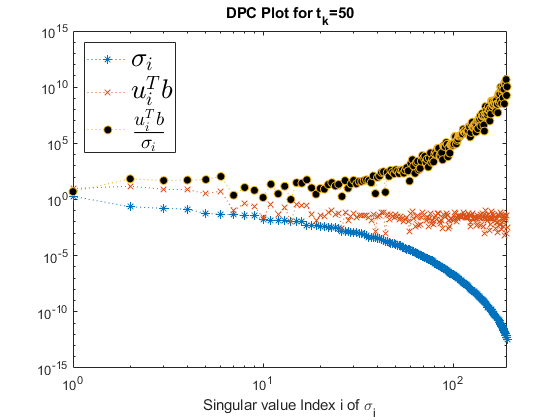
\includegraphics[width=0.8\textwidth]{../images/PicardPlot.png}
\caption{A sample Picard plot}\label{fig:PicardPlot}
\end{figure}

In ill-posed problems such as ECGI, there arises a point where singular values decay to zero faster than the data space coefficients and the computed solution is dominated by the smallest singular values and result in the amplification of the noise component in the measurements, \textit{i.e.}, where DPC starts to fail. Therefore, to compute a satisfactory solution, useful singular values larger than the regularization parameter $\lambda$ must decay slower to zero than the $|u_i^Tb|$.  

\subsection{Pacing Site Localization}

\begin{figure}[h]
\centering
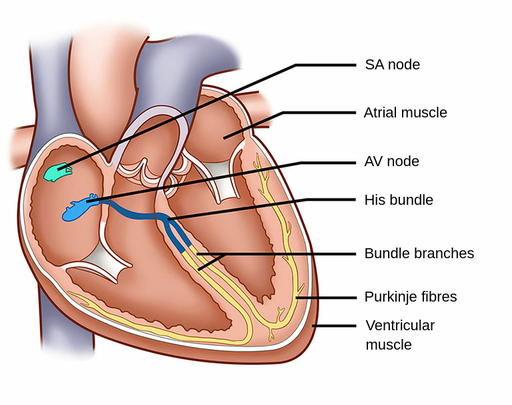
\includegraphics[width=0.8\textwidth]{../images/SA_Node.png}
\caption{Electrical anatomy of the heart}\label{fig:SANODE}
\end{figure}

In a healthy heart, Sinoatrial(SA) node is the natural pacemaker of the heart, \textit{i.e.}, the electrical signals start to propagate on the epicardial surface from this point. However, there may be some cardiac diseases where this point changes. Hence, it is a critical diagnosis factor for some diseases and locating this pacing site is critically important. The most common approach to this problem is to define a specific time instance, activation time(AT), for each beat paced from each node of the heart, and find the node having minimum AT is marked as the pacing site. Furthermore, regularization techniques can be utilized to enhance AT computation \cite*{erem2013using}.

\newpage
\subsection{Existent Regularization Parameter Choice Techniques}\label{subsec:paramselect}

The authors use 3 different techniques to compare the performance of their newly proposed selection algorithm. 

\subsubsection{Composite Residual and Smoothing Operator: CRESO}

CRESO \cite{colli1985mathematical} chooses the parameter that generates the first local maximum of the derivative of the residua and the constraint term. 

\begin{equation}
    C(\lambda) = \left\{ \frac{d}{d(\lambda^2)}(\lambda^2||a(\lambda)||^2) -  \frac{d}{d(\lambda^2)}||Ma(\lambda) - b||^2 \right\}
\end{equation}

\subsubsection{L-Curve}

L-curve is the log-log plot of residual($||Ma-b||$) and the constraint($||a(\lambda)||$) terms. To find optimum regularization parameter, the procedure proposed in \cite*{hansen1993use} is utilized and the point having the maximum curvature is marked as the optimal regularization parameter. 

\subsubsection{U-Curve}

U-Curve is relatively newer method that was proposed in \cite*{krawczyk2007regularization} whose cost function can be seen in \eqref{eq:ucurve}

\begin{equation}
    U(\lambda) = \frac{1}{||Ma(\lambda)-b||^2} + \frac{1}{||a(\lambda)||^2}
    \label{eq:ucurve}
\end{equation}

This cost function results in a U shaped function where the sides of the curve are where either the residual or the constraint term dominates. The minimum of the curve is chosen as the optimum regularization parameter. 

\newpage

\subsection{Automated Discrete Picard Condition (ADPC)}

Chamorro \textit{et al.} proposes an automated regularization parameter selection technique in \cite*{chamorro2017improving}. Using the approach mention in \nameref{subsec:DPC} section, the steps of the proposed algorithm is as follows: 

\begin{enumerate}
    \item Singular value decomposition of the system matrix is computed.
    \item For each time instant $t_k$, a polynomial of degree from 5 to 7 is fitted to the curve $p(i,log(|u_i^Tb_{t_k}|))_{t_k}$.
    \item For each $p_{t_k}$, the maximum singular value index $i$ is found, such that $log(\sigma_i) \geq p_{t_k}(i)$
    \item The ADPC regularization parameter is chosen as $\lambda = median({\lambda_{t_k}})$
\end{enumerate}


\section{Implementation}\label{sec:implementation}

This section comparatively explains how different datasets and methods are utilized in the original study and the reimplementation with a new experimental setup. 

\subsection{Datasets}

\subsubsection{Original Study}

The authors of the original study utilized a simulated dataset. They used eight different activation patterns:
\begin{itemize}
    \item 4 single site pacing in various locations in heart.
    \item 4 single spiral waves
\end{itemize}
The torso model was an anisotropic conductor one with 1 mm spatial resolution. The heart model consisted of left and right ventricles with 0.2 mm spatial resolution and fiber orientations were taken into account as an inhomogeneous conductivity. Both anatomies were based on MRI data and temporal resolution of the Ten Tusscher \cite*{ten2004model} model was 1 ms.

\subsubsection{Reimplementation}

I used the tank-torso preparation data from Utah experiments where the ground truth epicardial potential data were recorded \cite*{macleod1995electrocardiographic}. Already having the ground-truth epicardial potential matrix $X_{n_{nodes},t}$ where $n_{nodes}$ is the number of leads in the epicardial surface and $t$ is the number of time instances, BSPM data $Y$ is generated by the forward model in Section \ref{subsec:modelreimplement} and then corrupted by 30 dB SNR noise where SNR is calculated as follows:
\begin{itemize}
    \item Noise free $Y$ is obtained by applying the forward model operator (A) obtained via BEM: $Y = AX$
    \item Average power of the noise calculated as $P_{avg} = \frac{||Y(:)||_2}{\sqrt{n_{nodes} \times t}}$
    \item Then standard deviation of the noise for each lead is calculated using the formula $SNR = log(\frac{P_{avg}^2}{\sigma_n^2})$ where $\sigma_n$ is the standard deviation of the noise
    \item Finally, the mean of the generated noise is subtracted from itself and scaled with $\frac{||noise(:)||_2}{\sqrt{n_{nodes} \times t}}\sigma_n$ to achieve 0 mean noise with the desired SNR for each heart lead. 
\end{itemize}

\subsection{Model Generation} \label{subsec:modelgeneration}

\subsubsection{Original Study}

The authors used the MFS solutions model explained in Section \nameref{subsec:MFS}.

\subsubsection{Reimplementation}\label{subsec:modelreimplement}

In the reimplementation of the study, BEM is used to construct the forward model. The geometries were based on the torso tank experiments in \cite{macleod1995electrocardiographic}. Since BSPM is generated by the ground truth models, one should use a different inverse model to avoid inverse crimes. Hence, while the forward model is generated using a more realistic conductivity distribution by adding the lungs into the torso, lungs were removed out of the torso and a homogenous heart-torso model is utilized in the generation of the model. 

\begin{figure}[h!]
    \centering
    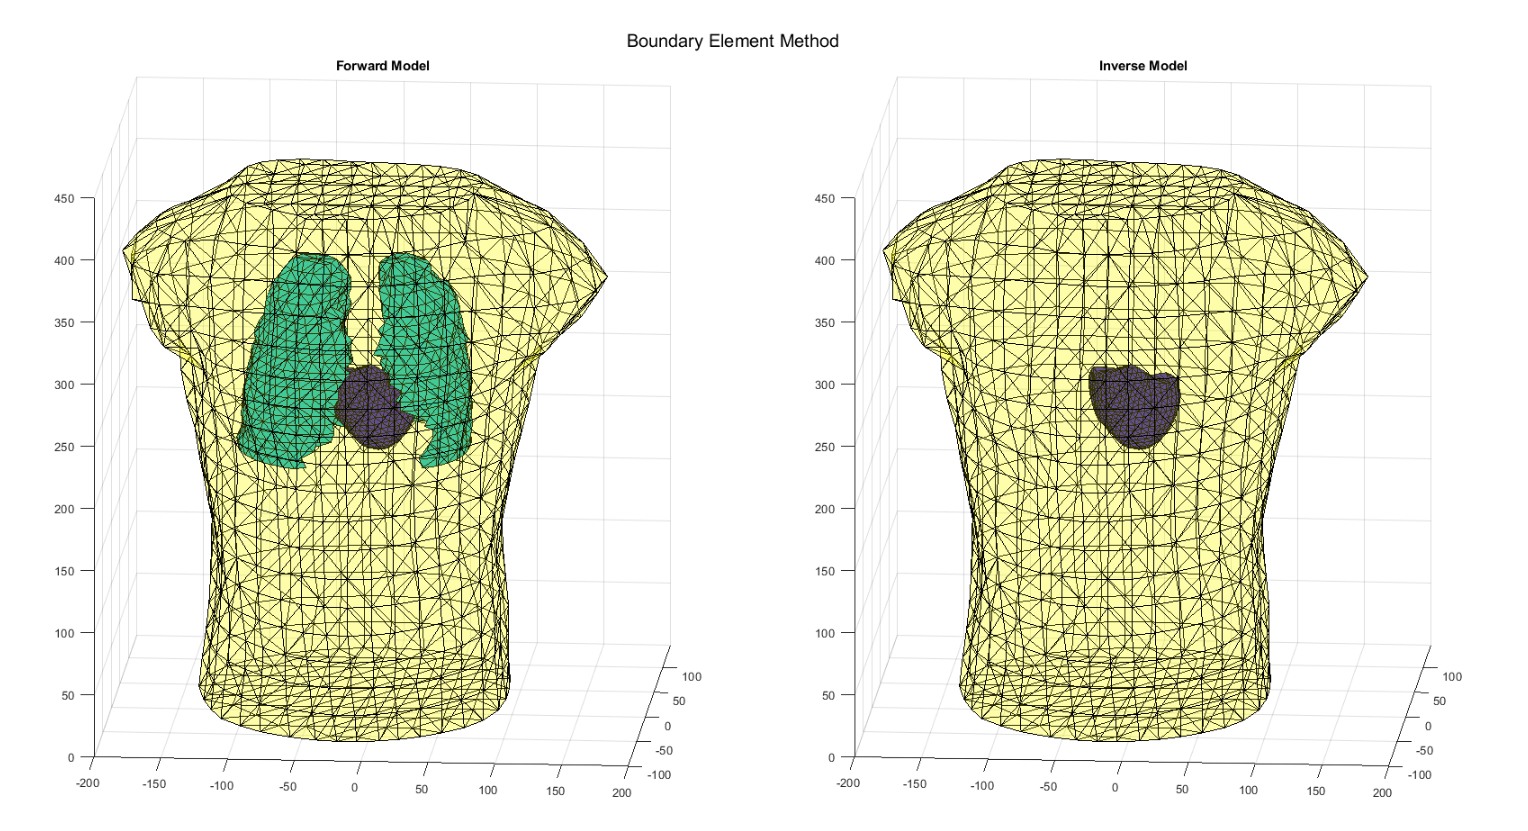
\includegraphics[width=0.8\textwidth]{../images/BEM.png}
    \caption{Forward and Inverse models generated with Boundary Element Method}\label{fig:mylabel}
\end{figure}
    
\subsection{Implementation of the Inverse Solution Computation}

To compute the inverse solution, Tikhonov-SVD expression given in \eqref{eq:tikhsvd} is utilized by processing the measurement matrix frame by frame with different forward and inverse models mentioned in \nameref{subsec:modelgeneration}, both in the original study and reimplemented version. In the reimplementation, I have modified the code from the codebase of \href{http://hrl.eee.metu.edu.tr/}{METU Heart Research Laboratory \faExternalLink*} for L-Curve optimization, noise generation which also includes the activation time generation from UTAH SCI\cite*{ActDetect}, and implemented all the remaining software including ADPC method and visualizations on MATLAB R2021b (The Mathworks, Inc., Massachusetts, United States). For visualizations, Gramm \cite*{morel2018gramm} is used. 

\subsubsection{L-Curve Implementation}

The line search conducted for L-curve choice of regularization parameter is conducted from $min(\sigma_1\cdot 16*\epsilon, \sigma_{smallest})$ to the maximum singular value $\sigma_i$ for 200 points in an exponential manner, and L-Curve is formed. Then the point having the maximum curvature is computed as described in \cite*{hansen1993use}.



\newpage

\section{Results and Discussion}\label{sec:discussion}

\subsection{Evaluation metrics}

In both implementations of ADPC, Pearson's Correlation Coefficient and Relative Error metrics are utilized in the temporal direction of the reconstruction, \textit{i.e.}, the beats recorded from different nodes of the heart and the reconstructed ones are compared for fixed locations. 

\begin{equation}
    Relative Error: \frac{||x-\hat{x}||_2}{||x||_2}
\end{equation}

\begin{equation}
    Pearson's Correlation Coefficient: \frac{n\sum x \hat{x} - n \sum x \sum y}{\sqrt{n\sum x^2 - (\sum x)^2}\sqrt{n\sum {\hat{x}}^2 - (\sum \hat{x})^2}}
\end{equation}

\subsection{Original Study}

\begin{table}[h]
\centering
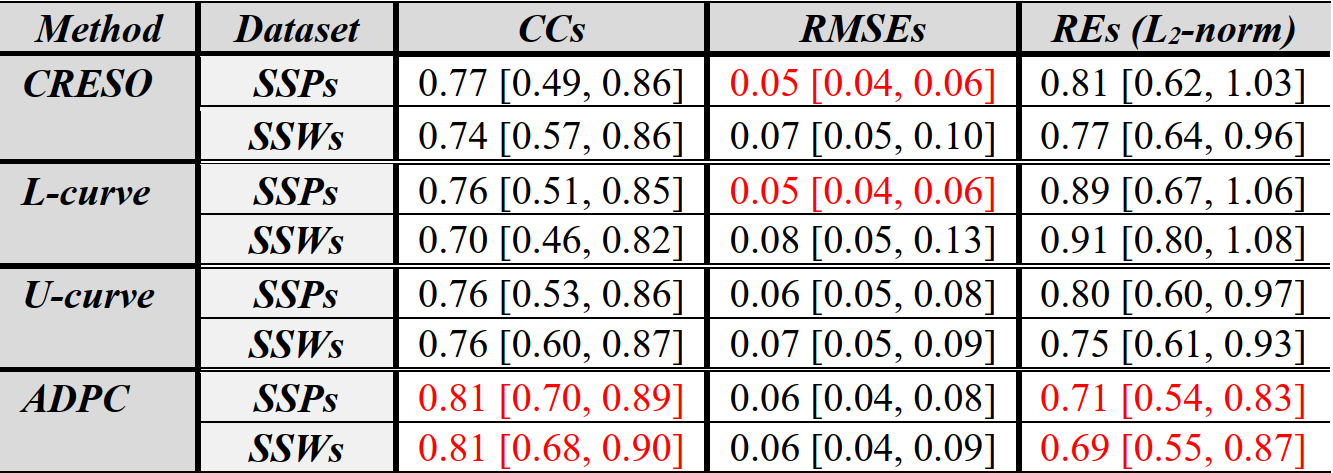
\includegraphics[width=0.8\textwidth]{../images/RecTable.png}
\caption{\label{tab:tabname}Reconstruction comparisons from the original paper}
\end{table}

\begin{table}[h]
    \centering
    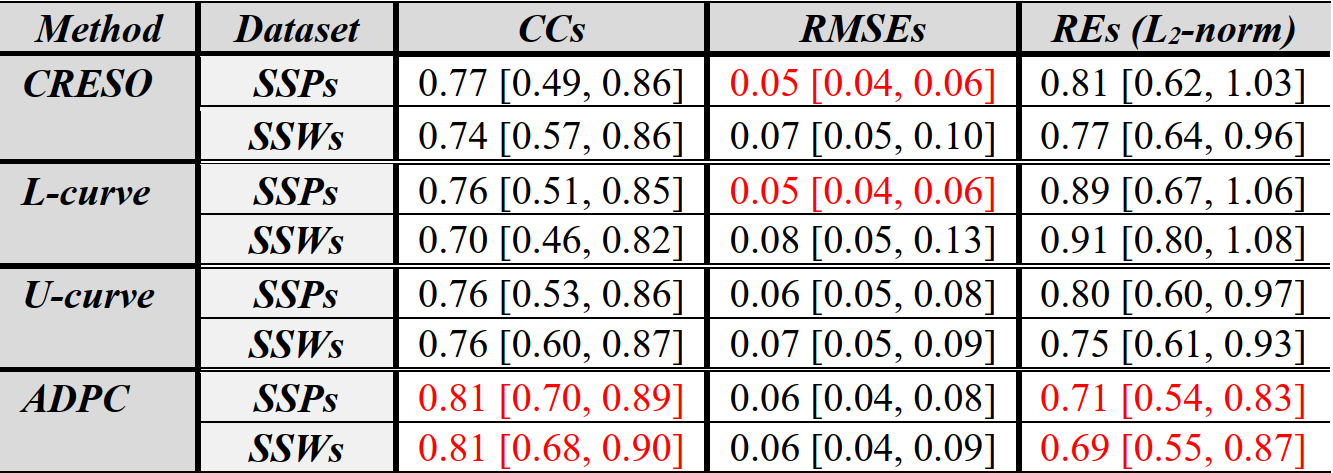
\includegraphics[width=0.8\textwidth]{../images/RecTable.png}
    \caption{\label{tab:tabname}Activation Time comparisons from the original paper}
\end{table}



\newpage
\printbibliography
\end{document}